\def\fasterrcnn{
    \subsubsection{Mô hình Faster R-CNN}
    Được lấy động lực từ mô hình Fast R-CNN, nhóm tác giả đã nghiên cứu và phát triển mô hình Faster R-CNN \cite{ren2015faster} với trung tâm là kiến trúc mô hình Region Proposal Network (gọi tắt là RPN).
    Mô hình Region Proposal Network được kỳ vọng sẽ thay thế hoàn toàn các thuật toán như Selective Search trong thành phần Region proposals module của các mô hình two-stage giải quyết bài toán object detection.
    Việc thay thế các thuật toán bằng một kiến trúc deep learning hướng đến việc cải thiện không chỉ tốc độ của mô hình mà còn cải thiện về độ chính xác. \\

    \noindent
    \textbf{\textit{Kiến trúc mô hình Region Proposal Network}} \\
    Mô hình RPN nhận đầu vào là ảnh với kích thước bất kỳ và trả đầu ra là toạ độ của các khu vực và xác suất khu vực đó là đối tượng nào trong các lớp đối tượng.
    Nhằm tiết kiệm chi phí tính toán, mô hình RPN dùng chung phần Feature extraction module với Fast R-CNN.
    Sau khi đưa ảnh qua Feature extraction module và thu được đặc trưng của ảnh đó, mô hình RPN trượt một sliding window trên đặc trưng.
    Và tại mỗi vị trí của sliding window trên đặc trưng, mô hình RPN tạo ra các khu vực đề xuất gọi là các anchor.
    \begin{figure}[H]
        \centering
        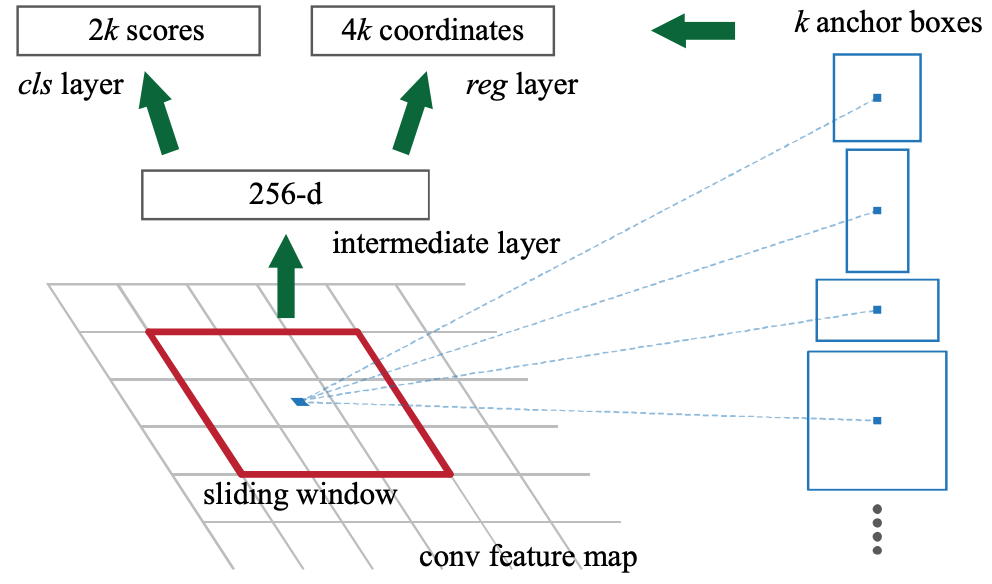
\includegraphics[width=13cm] {images/faster_rcnn_rpn}
        \caption{Kiến trúc mô hình Region Proposal Network (Nguồn: \cite{ren2015faster})}
        \label{fig:faster_rcnn_rpn}
    \end{figure}

    \noindent
    Nhóm tác giả xây dựng xây dựng phương pháp đề xuất các anchor dựa trên kích thước và tỷ lệ giữa chiều dài và chiều rộng của anchor.
    Cụ thể, với mỗi sliding window, nhóm tác giả đề xuất ba kích thước của anchor và ba tỷ lệ giữa chiều dài và chiều rộng của anchor, từ đó, ta có chín anchor với mỗi sliding window.
    Trên một đặc trưng của ảnh có kích thước $W x H$, ta sẽ thu được $W x H x k$ anchor.

    \noindent
    \textbf{\textit{Sự kết hợp giữa mô hình Region Proposal Network và Fast R-CNN}} \\

    \begin{figure}[H]
        \centering
        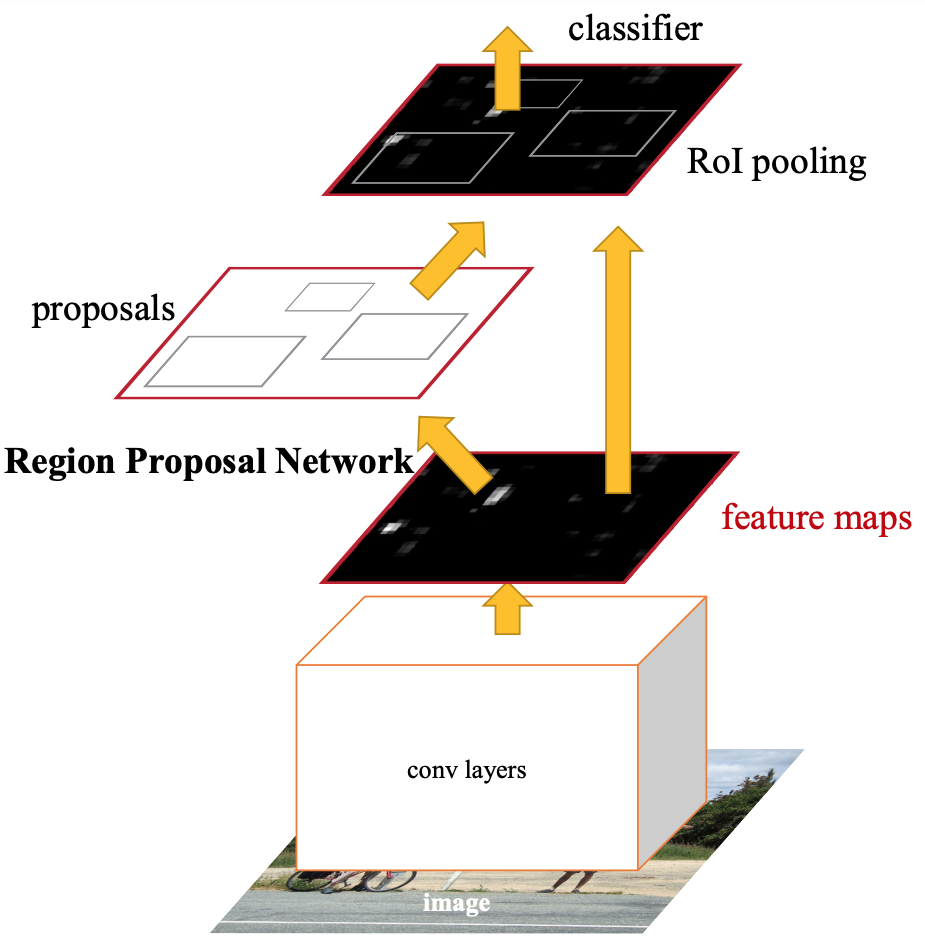
\includegraphics[width=13cm] {images/faster_rcnn_model}
        \caption{Toàn cảnh sự kết hợp của mô hình Region Proposal Network và Fast R-CNN tạo ra mô hình Faster R-CNN (Nguồn: \cite{ren2015faster})}
        \label{fig:faster_model}
    \end{figure}

    \noindent
    \textbf{\textit{Kết quả của mô hình Faster R-CNN}} \\
}